%!TEX root=paper.tex

\section{WebRT: Smart Web Browser Runtime Optimizing for Energy-Efficiency}
\label{sec:runtime}

Today's mobile processors are becoming extremely heterogeneous. They often combine general-purpose cores that have different performance and energy characteristics~\cite{single-ISA} (e.g., asymmetric chip-multiprocessor architecture) with special-purpose domain-specific cores (e.g., \webcore). While the hardware upheaval promises performance and energy improvements for the mobile Web, current Web runtime systems are not designed to fully exploit the capability of the underlying hardware. The main bottleneck is that current runtime-architecture interface merely exposes the hardware as a monolithic sequential execution model to the runtime system while hiding many architecture-level details. Without having a full visibility of the hardware details, current Web runtimes often lead to energy-inefficient decisions or violate user QoS requirement.

%While \greenweb APIs specify \textit{what} QoS type and QoS target that users expect, it is the job of the runtime substrate, i.e., the Web browser, to determine \textit{how} user QoS expectations are satisfied in an energy-efficient manner. In the Web stack, the Web browser acts as the runtime system of Web applications by translating and executing Web applications on the fly, similar to what JVM acts with respect to Java applications. Traditional Web browser designs have been primarily focused on functionality, correctness~\cite{atlantis}, and performance~\cite{ParallelBrowser} while largely neglecting its role in energy efficiency optimizations. 

To bridge the widening gap between the architecture complexity and the architecture-agnostic runtime system, I propose to enhance the existing runtime-architecture interface by exposing architecture details to the Web runtime. I specifically focus on the ACMP architecture~\cite{acmp, single-ISA} as the hardware substrate. ACMP is long known to provide a large performance-energy trade-off space, and is already widely used in today's mobile systems~\cite{big-little-future, exynos5biglittle}. Leveraging the enhanced interface, I propose \webrt, a Web runtime that minimizes energy while guaranteeing satisfactory user QoS experience by scheduling Web application executions using proper ACMP configurations.

In the rest of this section, I first provide an overview of \webrt (\Sect{sec:runtime:overview}). I discuss that optimizing energy consumption while delivering desirable user experience requires us first to understand the nature of different user interactions and to devise different optimization schemes accordingly. Specifically, I introduce a user-application interaction model called LTM. LTM captures three fundamental user interactions in mobile Web applications--Loading, Tapping, and Moving--and provides a framework for reasoning about different energy optimization strategies. I then describe \webrt's two critical components. The first component is the webpage-aware scheduler that targets the loading (L) process of a Web application (\Sect{sec:runtime:load}), and the second component is the event-based scheduler that targets the touching (T) and moving (M) interactions (\Sect{sec:runtime:ebs}). Finally, I compare the contrast \webrt with prior work on software support for mobile Web (\Sect{sec:runtime:related}).

\subsection{WebRT Overview}
\label{sec:runtime:overview}

An ACMP consists of cores with different microarchitectures, such as out-of-order and in-order. Each core has a variety of frequency settings. Different core and frequency combinations provide a large trade-off space between performance and energy. The objective of our ACMP-based \webrt is to find an ideal ACMP configuration (i.e., a $\langle core, frequency \rangle$ tuple) that minimizes the energy consumption while guaranteeing an acceptable responsive time when a user interaction happens.

To systematically analyze user interactions in mobile Web applications, we introduce a simple conceptual model called LTM, which captures three primitive user interaction forms: loading application page (L), tapping the display (T), and moving a finger on the display (M). The three interactions cover a majority of human-computer interactions on mobile devices: every application requires a loading phase (L), and post-loading interactions on mobile devices are mostly performed in the form of finger tapping (T) or finger moving (M).
%Specifically, moving could be manifested in various ways, such as scrolling, swiping, or even drawing a picture.

The prediction strategy for Loading needs to be different from that for Touching and Moving. The fundamental difference is that Loading occurs only once per usage session while Touching and Moving interactions occur repetitively throughout the entire Web application usage session. As a result, it is possible to make the prediction for the Touching and Moving interactions based on the history information within the same usage session. For Loading, however, every application loading is likely different from the previous one, and as such we can not make predictions based on previous loadings of (potentially different) applications. Instead, we have to make prediction based on the particular content of a given Web application. I now discuss the \webrt component that targets the Loading (\Sect{sec:runtime:load}) and Touching and Moving interactions (\Sect{sec:runtime:ebs}) separately.

\subsection{Webpage-aware Scheduling}
\label{sec:runtime:load}

\begin{table}[t]
\centering
\captionsetup{width=.7\columnwidth}
\renewcommand*{\arraystretch}{1.05}
\renewcommand*{\tabcolsep}{20pt}
\resizebox{.7\columnwidth}{!}{
\begin{tabular}{ll}
\toprule[0.15em]
\multicolumn{1}{l}{\bigstrut\textbf{Category}} & \multicolumn{1}{l}{\textbf{Model Predictors}}\\
\midrule[0.05em]
\multicolumn{1}{l}{\multirow{3}{*}{Webpage primitive: HTML}}
                &       Number of each tag \\
                &       Number of each attribute\\
                &       Number of DOM tree node\\
\midrule[0.05em]
\multicolumn{1}{l}{\multirow{3}{*}{Webpage primitive: CSS}}
                &       Number of rules \\
                &       Number of each selector pattern\\
                &       Number of each property \\
\midrule[0.05em]
\multicolumn{1}{l}{\multirow{2}{*}{Content-dependent}}
                &       Total image size \\
                &       Total webpage size \\
\bottomrule[0.15em]
\end{tabular}
}
\caption{\small Model Predictors}
\label{tab:feat_list}
\end{table}

In this section, we show that it is possible to predict the webpage load time and energy consumption using merely webpage-inherent characteristics. This prediction scheme had two advantages. First, it does not rely on any previous webpage loading history information and is based completely on each webpage's inherent characteristics. Second, the prediction is performed at the webpage parsing time which happens at the very beginning of the loading process, and as such allows enough time for energy optimizations. Based on such predictions, we propose a webpage-aware scheduler as a \webrt component that predicts the ACMP configuration for webpage loading in order to minimize energy consumption while meeting a specified cut-off latency.

\paragraph{Model Derivation} We find that regression models provide sufficient accuracy to predict the webpage load time and energy consumption. A regression model is a mathematical function between a set of predictors and a response. Within our context, the response is either the webpage's load time or energy consumption in loading the webpage. The predictors are a set of webpage characteristics. We also require a number of sampling observations to train the model. The linear regression is the basic regression technique and is the premise for advanced ones. Therefore, we first provide fundamentals of linear regression modeling. We then identify the predictors to the model and obtain a set of sampling observations in order to derive the linear model. After that, we describe how the different insights gathered in the previous section on webpage characteristics led us to refine the basic linear model.

The linear regression model models a webpage's load time and energy consumption (responses) as a linear combination of various webpage characteristics (predictors), formulated as: $y = \beta_0 + \sum_{i=1}^{p} x_i \beta_i$ where \textit{y} denotes the response, \textit{$x = x_{1},...,x_{p}$} denote \textit{p} predictors, and \textit{$\beta = \beta_{0},...,\beta_{p}$} denote corresponding coefficients of each predictor. The \textit{least squares method} is used to identify the best-fitting $\beta$ that minimizes the residual sum of squares (RSS)~\cite{ESL}.

We consider two types of predictors. The first type includes the \textit{webpage-inherent} primitives such as the number of HTML tags. In addition, we must also consider the impact of \textit{content-dependent characteristics} such as image size and the total size of a webpage. These characteristics are coarse-grained metrics that are independent of webpage structures but which influence the load time and energy of rendering. We summarize these features in \Tbl{tab:feat_list}. In total, we consider 376 predictors. We require a number of sampling observations to construct the regression models. In total, we obtain 2,500 sampling observations, for which we measure both webpage load time and energy consumption simultaneously on the Cortex-A9 processor running at 1.2 GHz.

We apply a set of techniques to improve the accuracy of the basic linear model. The most significant one is based on the observation that the true relationship between the response and all predictors is strictly linear as assumed by simple linear models.  One effective method to model nonlinearity is to fit data with \textit{restricted spline} functions that are piecewise polynomial functions but which force linear fitting beyond the first and last knots~\cite{ESL}.
 
\paragraph{Model Evaluation} To validate the model, we obtain 2,500 observations in addition to the 2,500 observations used in deriving the model. Overall, the performance model predicts 73.0\% of the webpages within 10\% error and 94.0\% webpages within 20\% error. Similarly, the energy model predicts 70.0\% of the webpages within 10\% error and 91.8\% webpages within 20\% error. Overall, we find the model accuracy to be acceptable.

\paragraph{Scheduler} During the parsing stage, the webpage-aware scheduler extracts webpage characteristics, and feeds them into the prediction models to estimate the webpage load time and energy consumption under different core and frequency configurations.  On the basis of these predictions, the scheduler then identifies the configuration (if possible) that meets the cut-off latency with minimal energy consumption. If no such configuration is found, the webpage is scheduled to the big core with the highest frequency for the best possible performance.

\paragraph{Overheads} The scheduler accounts for scheduling overheads, which consist of two components: the prediction overhead and the overhead of changing the architecture configuration (i.e, big/little core migration and/or frequency scaling). The prediction cost is negligible. We assume an 100~$\mu$s overhead for frequency scaling and a 20~$\mu$s overhead for core migration, as indicated in whitepapers released by ARM~\cite{arm-bl-sw-wp, arm-bl-wp}. Note that the overhead of switching architecture configuration also applies to the event-based scheduling discussed below.

\subsection{Event-based Scheduling}
\label{sec:runtime:ebs}

I propose event-based scheduling (EBS) as the mechanism to optimize energy-efficiency for the Touching (T) and Moving (M) interactions. Each T or M interaction is internally translated to an application event. EBS is based on the observation that a T or M event may occur repetitively throughout a Web application usage session such that it is possible to predict the ideal architecture configuration of an event based on its history information of performance and energy consumption. I first provide an overview of EBS and discuss several key implementation details.

\paragraph{Overview} The key idea of identifying an event's ideal execution configuration is to build a performance model and an energy model. They predict an event's latency and energy consumption under any core and frequency combination. With the two models, EBS sweeps all possible core and frequency combinations and selects the one that meets the QoS target with minimal energy.

The scheduler consists of a simple dispatch frontend and scheduling backend as illustrated in~\Fig{fig:runtime}. The frontend \textit{Dispatch} unit extracts relevant event information, and passes it to the backend. The backend consists of a \textit{Detector}, a \textit{Model Constructor} and a \textit{QoS Monitor}. The detector
automatically identifies each event's QoS requirement. In its simplest form, the detector assumes a default latency target, such as 100~ms, for each event. If an event is annotated with programmer-guided QoS hints such as those enabled by the \greenweb language extensions as I will discuss in \Sect{sec:lang}, the detector can also extract the specified QoS information from the application. The model constructor builds a performance and energy model for each event. The models and event QoS information are then fed into the QoS monitor, which predicts the architecture configuration for executing an event while meeting the specified QoS target.

During application execution, the QoS monitor keeps monitoring event execution time and energy consumption on the hardware and uses the information to adjust its prediction and scheduling decisions on the fly, similar to conventional feedback-driven optimizations~\cite{FDO}. Intuitively, it is possible for the performance and energy models to underpredict or overpredict the architecture configuration. Under such circumstances, the monitor can decide to tune the predicted frequency or transition between big and little cores. If the models are deemed completely unusable, the monitor informs the model constructor to recalibrate the models. We now describe some key implementation details of the QoS monitor operations.

\begin{figure}[t]
  \centering
  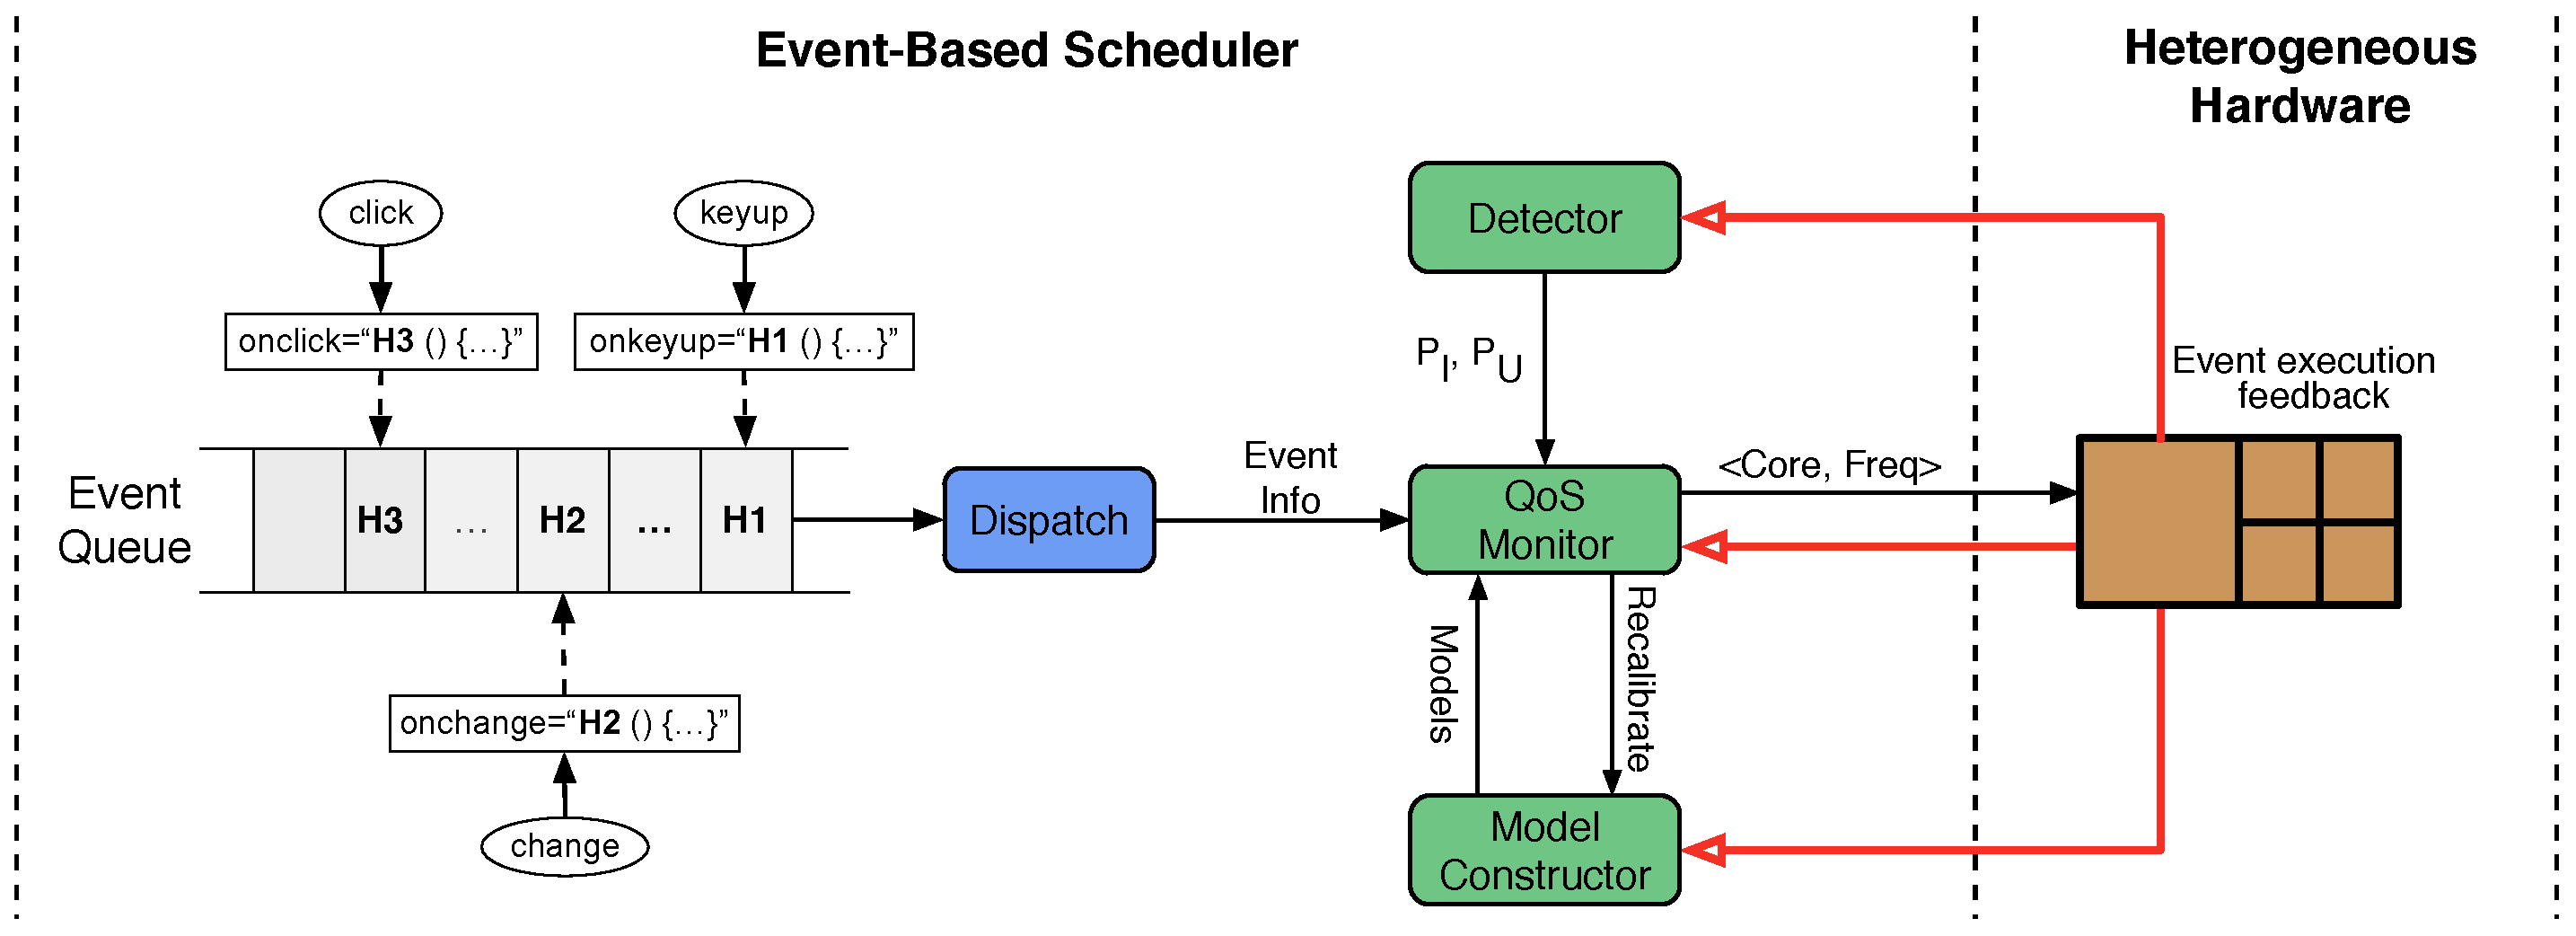
\includegraphics[trim=0 0 0 0, clip, width=.9\columnwidth]{runtime}
  \caption{\small{The EBS runtime framework.}}
  \label{fig:runtime}
\end{figure}

\paragraph{Performance Model} The performance model predicts event execution time under different frequencies. We use the classical DVFS analytical model initially proposed in~\cite{dvfs_model}, and employed in subsequent work, such as~\cite{dvfs_power}:
\begin{align*}
Execution\,\,\,time = T_{memory} + N_{dependent}/f
\end{align*}
where $f$ is the CPU frequency, $T_{memory}$ is the absolute memory access time that does not change with respect to the CPU frequency, and $N_{dependent}$ is the number of CPU cycles that are not overlapped with the memory accesses.

Strictly speaking, $N_{dependent}$ is a function of $f$. However, precisely constructing a model that varies $N_{dependent}$ with $f$ is complex and introduces a large calibration overhead at runtime. In our experiments, we find that it is feasible and necessary to trade model precision for performance. In particular, we find that treating $N_{dependent}$ as a constant is sufficient in our case. Given this simplification, the model constructor builds the model by profiling twice, one at the maximum frequency and one at the minimum frequency.

\paragraph{Energy Model} The energy model predicts the energy consumption of an event execution. We construct the energy model based on the performance model and the estimated power consumption. We derive the power estimation of all the core and frequency combinations by performing a profiling run and storing the results in a local power profile file that is read by the Web application upon every launch. Persisting the power profile file aligns with the Android standard~\cite{powerxml}. 

\paragraph{QoS Monitor's Operation} The QoS monitor constructs a deterministic finite automaton (DFA) for each event to keep track of what architectural configuration it needs to provide. The first two times an event is executed, the QoS monitor informs the model constructor to build the performance and energy models. The models let the monitor predict the architecture configuration during all subsequent executions of the event handler.

After the initial model construction, the QoS monitor keeps monitoring event execution in order to perform fine-grained tuning. Specifically, the monitor compares the measured event execution time with the QoS target. The monitor conservatively deems an event's model as overpredicting (or underpredicting) if the measured value is lower than 80\% (or higher than 90\%) of the QoS target. We empirically adopt these two threshold values because they are found to be effective in practice. Using a two-bit saturating counter, the monitor increases the frequency by 100~MHz or transitions from the little core to the big core if the model is underpredicting, or vice versa.

The monitor switches from fine-tuning an event handler's execution to recalibrating its model if it detects that the model is not performing well. We use a simple heuristic that is efficient in practice. If the model mispredicts (i.e., either underpredicts or overpredicts) more than four consecutive times, the monitor requests the model constructor to recalibrate.

\subsection{Related Work}
\label{sec:runtime:related}

\paragraph{Single ISA Heterogeneous Scheduling} The particular implementation of \webrt is an example of utilizing single-ISA heterogeneous systems for trading off performance with energy~\cite{single-ISA}. Nvidia's Kal-El~\cite{Tegra3} is a single-ISA heterogeneous system that integrates four high-frequency cores with one low-frequency core. ARM's proposed big.LITTLE system~\cite{big.little} contains an out-of-order Cortex-A15 processor and an in-order Cortex-A7 processor. ACMP architecture is already widely adopted in today's mobile SoCs shipped by major vendors. We expect our \webrt implementation to be readily applicable to commodity mobile hardware.

\webrt's prediction-based scheduling technique is similar to other recent heterogeneous scheduling proposals, such as PIE~\cite{PIE}. However, instead of relying on (micro)architecture- and system-level statistics for prediction, we capture the complex behavior of webpage characteristics using regression modeling, and accurately predict the webpage load time and energy consumption.

\paragraph{General Software Support for Web Optimizations} Most prior research focus on parallelizing browser tasks, such as parsing, CSS selection, etc.~\cite{ParallelBrowser, FTL, UCI, Parabix}. Although such parallelized algorithms can achieve speedups ranging from 4X to 80X for various browsing tasks, they typically do not scale well beyond four cores with the expense of potential energy inefficiency. Thus, while parallelization has potential in desktop systems, it is less favorable for mobile Web computing.

Thiagarajan~et al.~\cite{www-battery} break the Web browser's energy consumption into coarser-grained elements, such as CSS and Javascript behavior, and identify a few system- and application-level optimizations to improve the energy consumption of mobile Web browsing.  The optimizations they recommend, such as reorganizing JavaScript files and removing unnecessary CSS rules, are orthogonal and complementary to our webpage prediction and scheduling work.
%Other works analyze the power/energy consumption of the entire smartphone\cite{Carroll, Eprof, JamesHotchip}, whereas we focus on improving the energy-efficiency of the mobile processor in response to the demand for high-performance.

Another portion of software-level optimizations focuses on improving the execution model of the Web browser through asynchronous/multiprocess rendering, resource prefetching, smarter browser caching, etc.~\cite{pocketweb, Adrenaline, smart-caching, webkit2, firefox-spec_parsing}. All these techniques are orthogonal and can be integrated with my proposal, which primarily focused on the core rendering engine of a Web browser.

%\subsection{Preliminary Results}
%\label{sec:runtime:eval}
%
%In this section, we present preliminary experiment results of both the event-based scheduling~(\Sect{sec:runtime:eval:ebs}) and the webpage-aware scheduling~(\Sect{sec:runtime:eval:was}).
%
%\subsubsection{EBS Results}
%\label{sec:runtime:eval:ebs}
%
%\begin{table}[t]
%\centering
%\captionsetup{width=\columnwidth}
%\caption{\small List of applications. ``Time'' indicates interaction duration. ``Annotation'' indicates percentage of events that are annotated. ``Events'' indicates the amount of events triggered during full interaction. We only annotate and count events that are directly triggered by mobile user interactions.}
%\renewcommand*{\arraystretch}{1.2}
%\renewcommand*{\tabcolsep}{12pt}
%\resizebox{\columnwidth}{!}
%{
%\begin{tabular}{l r r r | l r r r}
%\toprule[0.15em]
%\bigstrut\textbf{Application}  & \bigstrut\textbf{Time}  & \bigstrut\textbf{Events} & \bigstrut\textbf{Annotation} & \bigstrut\textbf{Application}  & \bigstrut\textbf{Time}  & \bigstrut\textbf{Events} & \bigstrut\textbf{Annotation} \\
%\midrule[0.05em]
%BBC          & 0:86    & 60    &  20\%  & Amazon     & 0:36    & 101   &   33\%  \\
%Google      & 0:31    & 26    & 87.5\%  & Craigslist   & 0:25    & 22    & 84.6\%   \\
%CamanJS  & 0:49    & 24    & 100\%  & Paper.js     & 0:16    & 560    & 100\%  \\
%LZMA-JS   & 0:53    & 39    & 100\%  & Cnet          & 0:46    & 60    & 55.3\%  \\
%MSN          & 0:59    & 126   & 51.2\% & Goo.ne.jp   & 0:16    & 23    & 51.8\%   \\
%Todo         & 0:26    & 26    & 38.3\%  & W3Schools  & 0:64    & 59    & 100\%    \\
%\bottomrule[0.15em]
%\end{tabular}
%}
%\label{tab:app}
%\end{table}
%
%\paragraph{Application Selection} \Tbl{tab:app} shows the applications we use for evaluation. We crawl them using HTTrack~\cite{httrack} and host them on our own Web server to enable annotations (discussed later). We acknowledge that the network condition could be slightly better when accessing a local server. However, we believe it has minimal impact because many prior work has shown that computation dominates the performance and energy consumption for today's mobile Web applications~\cite{zhu2015role, huang2012close, big-little}. Overall, these applications cover a wide range of domains such as news, utility, etc., and are mostly among the top 200 websites as ranked by Alexa~\cite{alexa}.
%
%We perform a sequence of interactions on each application, and evaluate end-to-end behavior of EBS. Each sequence consists of a mix of touching and moving interactions and contains events with different QoS types and QoS targets. \Tbl{tab:app} shows the details of each interaction. On average, each interaction sequence triggers about 94 events and lasts about 43~s.
%
%We acknowledge that there are alternative ways to interact with each application. Thoroughly evaluating all the representative interactions with each application involves a large user study and is beyond the scope of this paper. However, we did perform our due diligence to make sure that the chosen interaction for each application is representative.
%
%\begin{figure*}[t]
%\centering
%\subfloat[\small{Energy consumptions normalized to \textit{Perf}. Lower is better.}]
%{
%  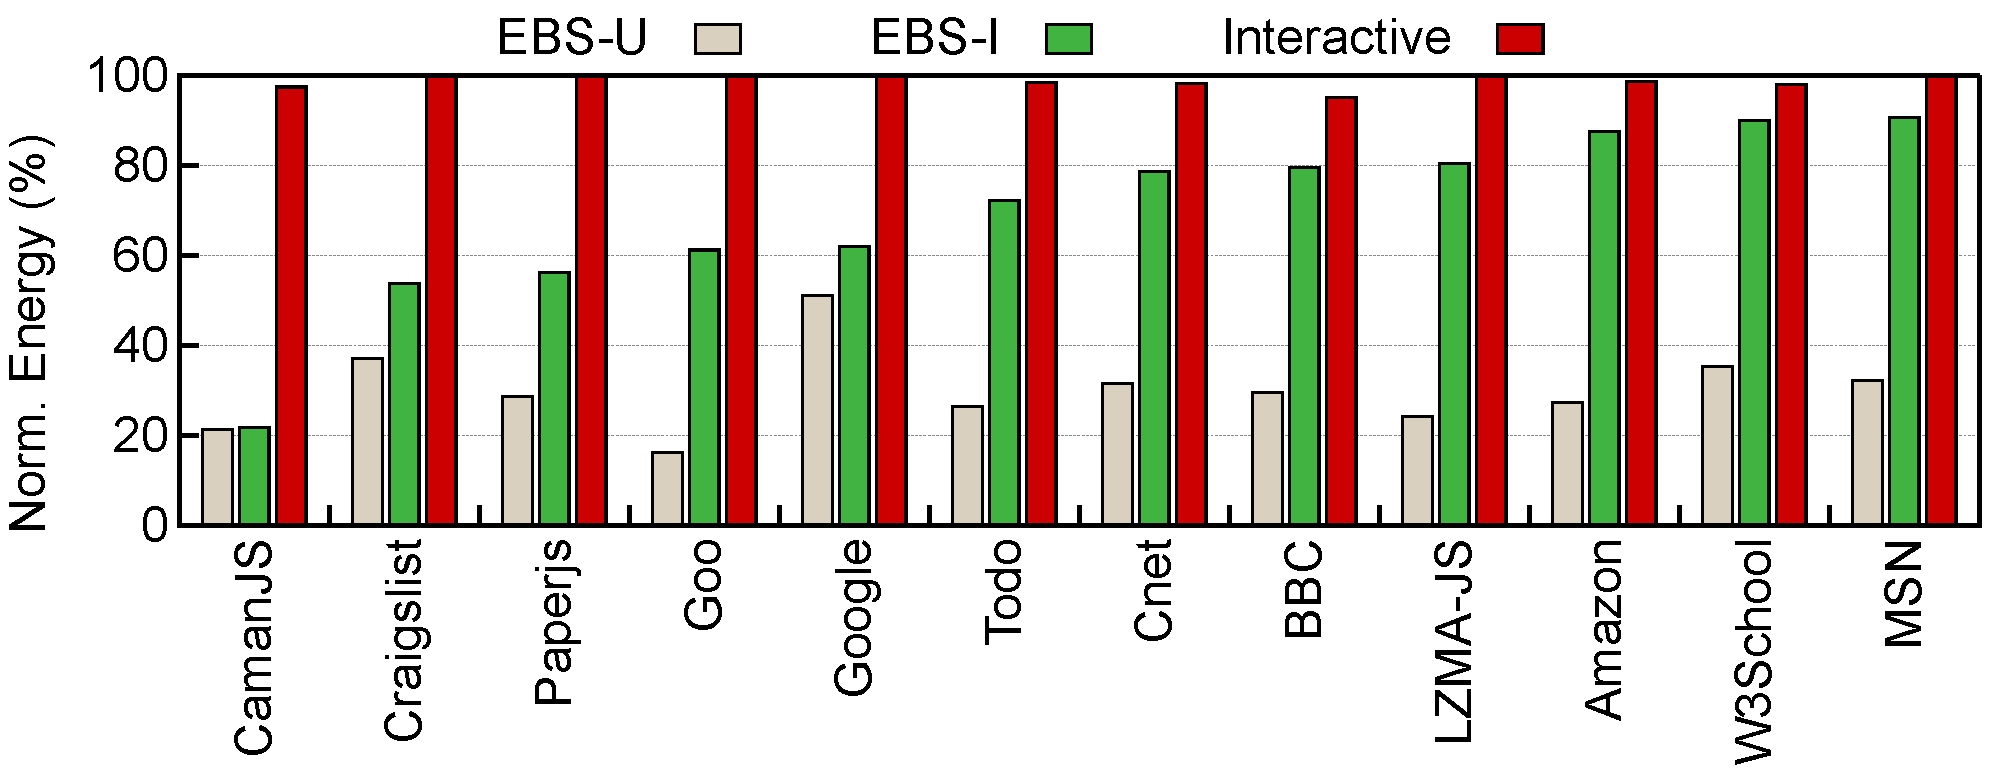
\includegraphics[trim=0 0 0 0, clip, width=0.7\columnwidth]{energy_results_f}
%  \label{fig:energy_results_f}
%}\\
%\subfloat[\small{QoS violation comparison under the imperceptible usage scenario.}]
%{
%  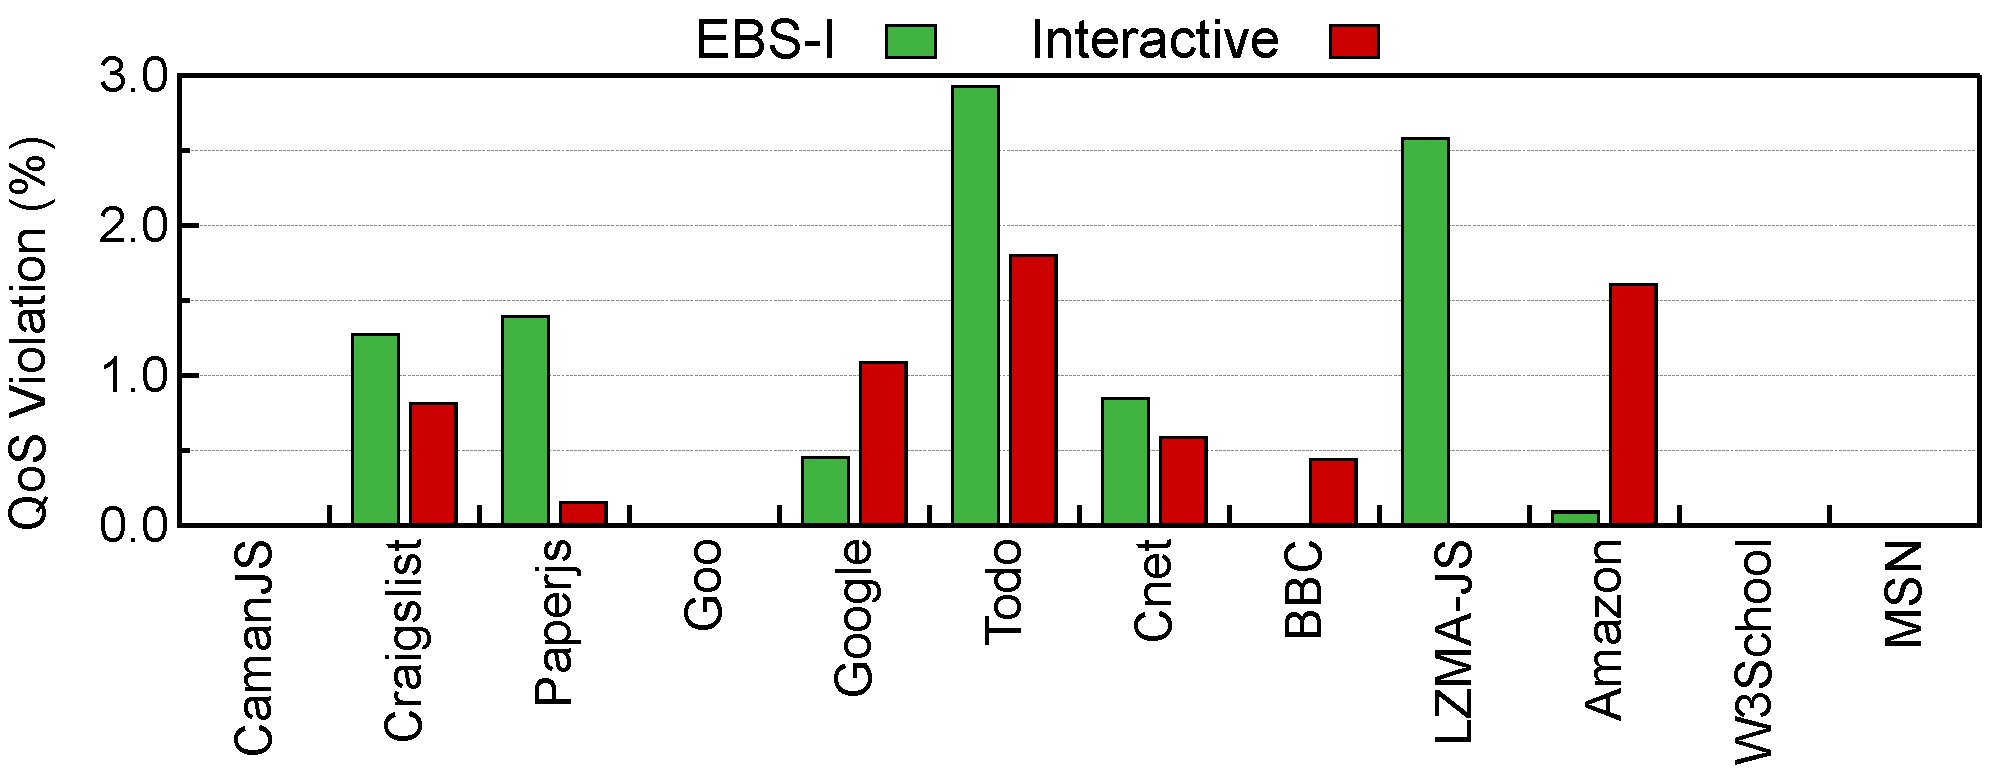
\includegraphics[trim=0 0 0 0, clip, width=0.4\columnwidth]{qos_pi_results_f}
%  \label{fig:qos_pi_results_f}
%}
%\hspace*{10pt}
%\subfloat[\small{QoS violation comparison under the usable usage scenario.}]
%{
%  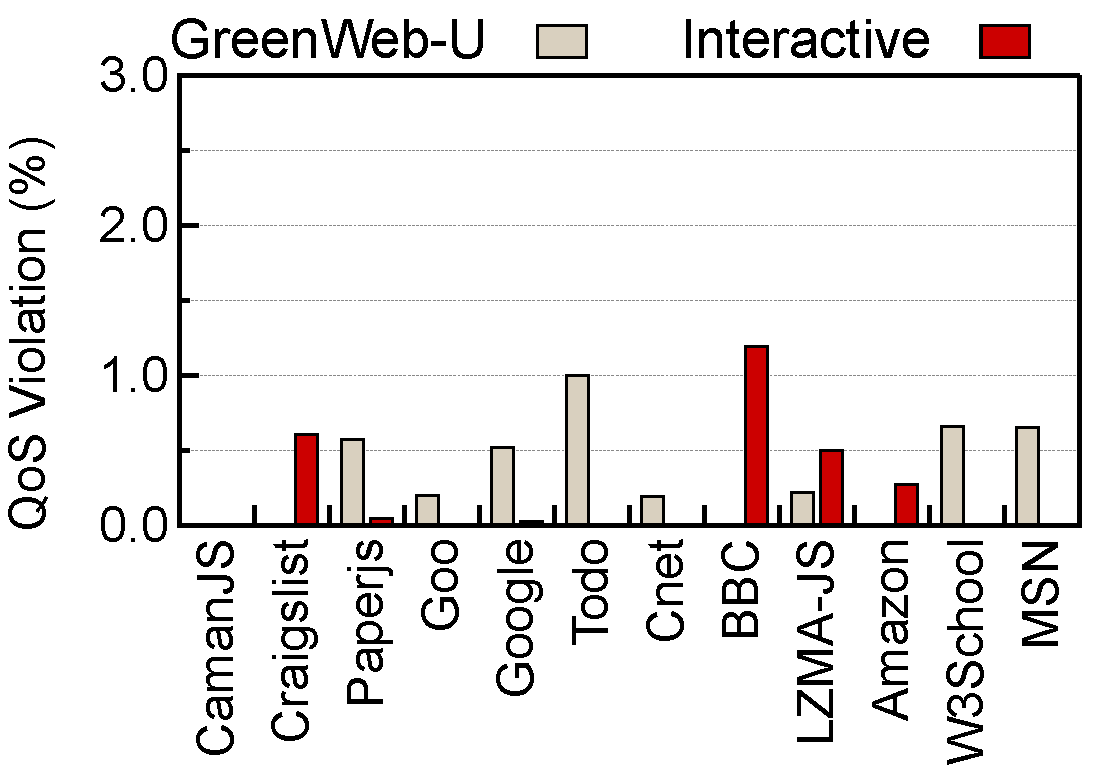
\includegraphics[trim=0 0 0 0, clip, width=0.4\columnwidth]{qos_pu_results_f}
%  \label{fig:qos_pu_results_f}
%}
%\captionsetup{width=.9\columnwidth}
%\caption{\small Full interaction results. Energy savings are normalized to \textit{Perf}. QoS violations are presented as additional violations on top of \textit{Perf}.}
%\label{fig:full_results}
%\end{figure*}
%
%\paragraph{Baseline} We compare EBS with two baselines:
%
%\begin{itemize}
%  \item \textit{Perf} is the policy that always runs the system at the peak performance, i.e., highest frequency in the big core in our setup. It is the standard policy for interactive applications to guarantee the best user QoS experience.
%
%  \item \textit{Interactive} is Android's default \texttt{interactive} CPU governor designed specifically for interactive usages. It maximizes performance when the CPU recovers from the idle state, and then dynamically changes CPU performance as CPU utilization varies~\cite{android_cpufreq}.
%\end{itemize}
%
%\paragraph{Usage Scenarios} Real-world user study over one year span from LiveLab~\cite{livelab} shows that mobile users often have to interact with devices under different battery conditions. Therefore, we evaluate \webrt under two major usage scenarios based on battery condition:
%
%\begin{itemize}
%  \item ``Imperceptible'' represents scenarios in which the battery budget is abundant and users expect high QoS experience. It corresponds to the imperceptible QoS experience discussed in \Sect{sec:lang:eqos}. The imperceptible performance threshold $T_I$ is used as the QoS target.
%
%  \item ``Usable'' represents scenarios in which the battery budget is tight and users could tolerate lower performance. It corresponds to the usable QoS experience. The usable performance threshold $T_U$ is used as the QoS target.
%\end{itemize}
%
%It is worth noting that \textit{Perf} and \textit{Interactive} behave the same independent of the usage scenario. \greenweb under these two scenarios are denoted by \textit{EBS-I} and \textit{EBS-U}, respectively, in the rest of the evaluation.
%
%\paragraph{Energy Savings} \Fig{fig:energy_results_f} shows the energy consumption of \textit{Interactive} and EBS. The results are normalized to \textit{Perf}. As compared to \textit{Interactive}, EBS achieves on average 21.2\% and 67.5\% energy saving under the imperceptible and usable usage scenarios, respectively.
%
%\textit{Interactive} consume energy close to \textit{Perf} across all applications, indicating that the Android \texttt{Interactive} governor is almost always operating at the peak performance. This is because user interactions, especially events with a ``continuous'' QoS type, typically generate a large volume of frames, which leads to high CPU utilization. \textit{Interactive} responds to the high CPU utilization by increasing CPU performance. With the QoS knowledge provided by developers, EBS can identify execution configurations that conserve energy while still meeting QoS requirements.
%
%\paragraph{QoS Violation} \Fig{fig:qos_pi_results_f} and \Fig{fig:qos_pu_results_f} show the QoS violation of \textit{Interactive} and EBS under the imperceptible and usable scenarios, respectively. On average, EBS introduces 0.8\% and 0.6\% more QoS violations than \textit{Perf} under the imperceptible and usable scenarios, respectively. The QoS violations are lower than in microbenchmarks because interaction duration gets longer and the QoS violations caused by profiling runs are amortized.
%
%Compared to \textit{Interactive}, EBS has similar, in some cases fewer, QoS violations. Considering the significant energy savings, we conclude that the
% QoS-aware EBS system can use energy more wisely by being aware of user QoS expectations. Overall, EBS achieves better energy efficiency than the 
%QoS-agnostic \textit{Interactive} scheme.
%
%\subsubsection{Webpage-aware Scheduler Results}
%\label{sec:runtime:eval:was}
%
%We compare the webpage-aware scheduling mechanism against an intelligent synthesized OS scheduler that performs on-demand DVFS on a heterogeneous system. The OS scheduler scales the frequency during a webpage load based on simple heuristics of system utilization~\cite{OS_DVFS1, OS_DVFS2}. It samples the CPU usage at a certain period and scales up the frequency if the average CPU usage in the previous sampling period is above a preset threshold, and vice versa. Because no Linux scheduler can yet perform heterogeneous scheduling across big/little cores, we synthesize such a scheduler by running the webpages under the ``on-demand'' cpufreq-governor~\cite{ondemand} on the big core and the little core, individually, and then choose the better result.
%
%\begin{figure}[t]
%\centering
%\subfloat[\small{Distribution of per webpage energy saving against the baseline.}]{
%    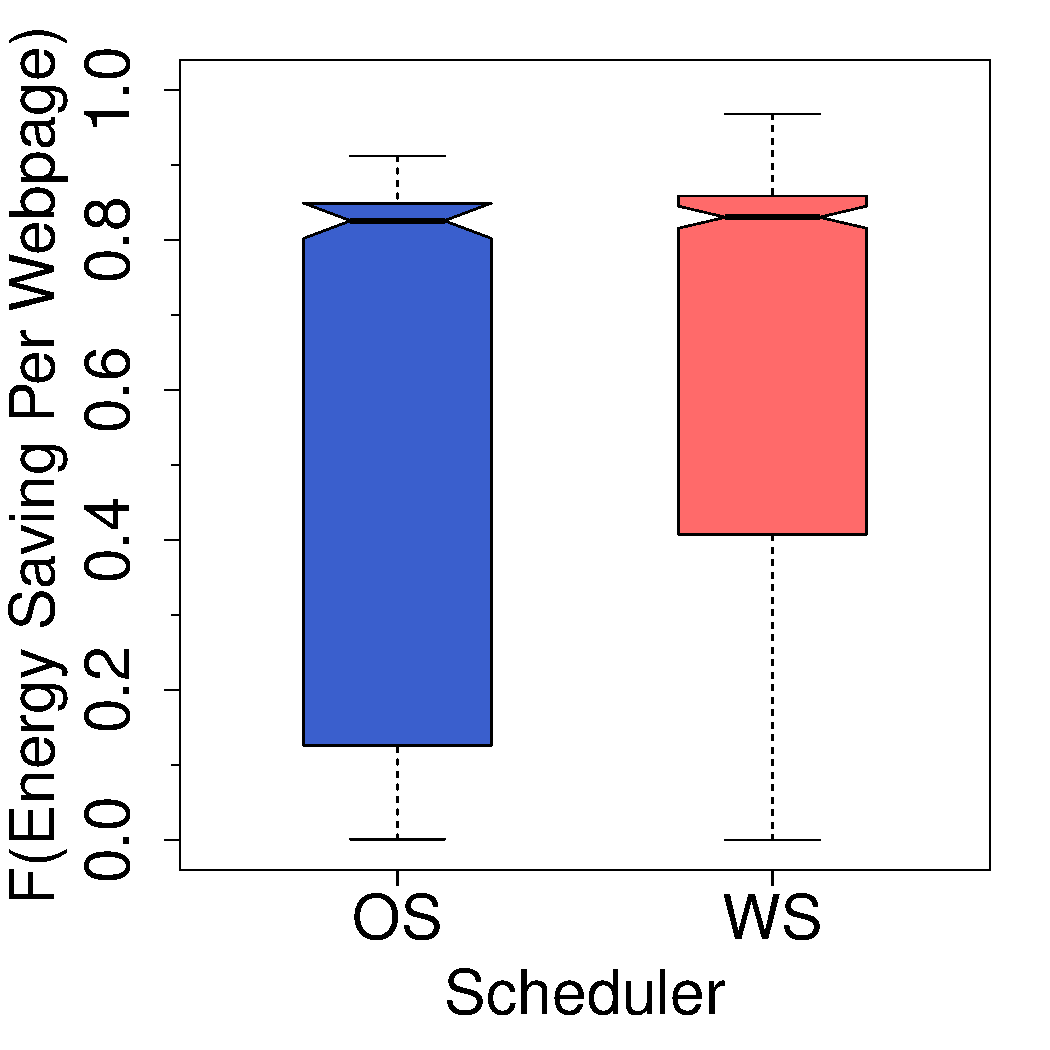
\includegraphics[trim=0 0 0 0, clip, width=.3\columnwidth]{boxplot}
%\label{fig:results_energy}
%}
%\hspace*{25pt}
%\subfloat[\small{Number of webpages that violate a 3-second cut-off latency.}]{
%    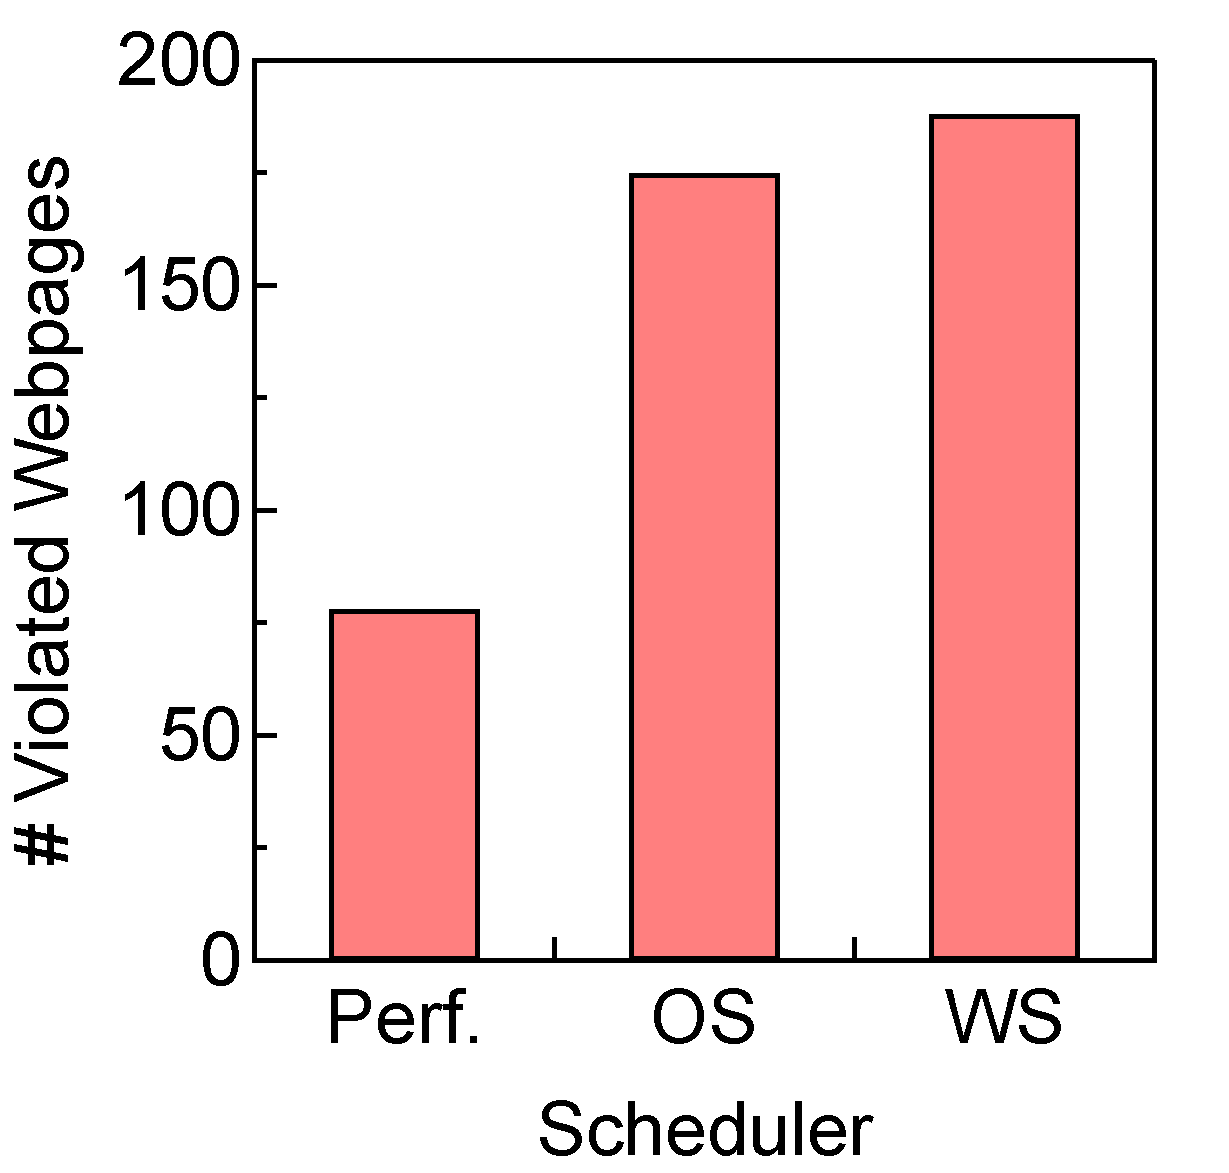
\includegraphics[trim=0 0 0 0, clip, width=.3\columnwidth]{results_cutoff}
%\label{fig:results_cutoff}
%}
%\caption{\small Evaluation of different scheduling strategies.}
%\label{fig:sched_results}
%\end{figure}
%
%We compare the two scheduling techniques with a baseline strategy that consistently yields the best performance. The baseline configuration is the big core~(A9) with its peak frequency~(1.2~GHz). We evaluate the same 2,500 webpages that we used to assess the accuracy of the regression models. Assuming a 3~second cut-off latency, \Fig{fig:results_energy} shows the boxplot of per-webpage energy savings under the webpage-aware and OS schedulers against the high-performance mode. Both schedulers achieve significant energy savings over the high-performance baseline, with a (geometric) average of 83.6\% and 83.0\%, respectively. This is because both schedulers can schedule webpages to the lower power core or lower frequency. The webpage-aware scheduler has a denser energy-saving distribution toward 100\% than the OS scheduler. On average, the webpage-aware scheduler reduces energy consumption by 8.6\% compared with the OS scheduler.
%
%Both the OS scheduler and the webpage-aware scheduler trade performance for better energy savings compared with the performance mode. We evaluate their behaviors more critically using the number of webpages that violate the cut-off latency under their operations. This data is shown in \Fig{fig:results_cutoff}. The performance mode violates only 3.5\% of the webpages with a 3~second cut-off latency because it always operates at peak computational capability. Both of the software schedulers perform slightly worse. Our mechanism, the webpage-aware scheduler, results in 7.6\% violations, which is only 0.6\% worse than the OS scheduler. However, on (geometric) average, our mechanism loads webpages 4.0\% faster than the OS scheduler.
